% !TEX root = ./Basilisk-oeStateEphem-20190426.tex


\begin{figure}[h]
	\centerline{
		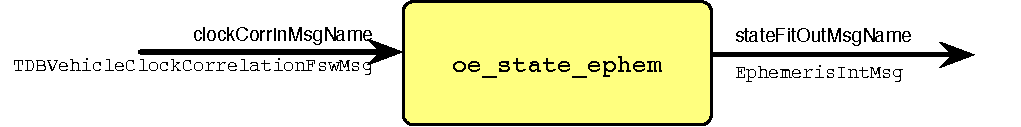
\includegraphics{Figures/moduleImg}
	}
	\caption{Illustration of the module input and output messages.}
	\label{fig:moduleImg}
\end{figure}


\section{Model Description}
The purpose of this module is to model a trajectory in space using a fitted set of Chebyshev coefficients.  As illustrated in Figure~\ref{fig:moduleImg}, there is a single input message which provides the ephemeris time associated with the vehicle on the trajectory, as well as vehicle time code information.  This is used to compute a corrected mission time used to compute the location on a given trajectory.

The output of the module is an ephemeris interface message which contains the inertial position vector $\leftexp{N}{\bm r}$ and inertial velocity $\leftexp{N}{\dot{\bm r}}$.  To model the trajectory  a Chebyshev polynomial approximation is used of the orbit elements.  The elements modeled include the radius at periapses $r_{p}$, the eccentricity $e$, the inclination angle $i$, the ascending node angle $\Omega$, the argument of periapses angle $\omega$ and an anomaly angle. The elements were chosen as they are defined finite quantities for ellipses, parabolas and hyperbolas.  The anomaly can can be the true anomaly directly (default), or the mean elliptical or mean hyperbolic angle depending on the value of the eccentricity $e$.  The input type is controlled within the Chebyshev record structure through the variable {\tt anomalyFlag}.  In all cases the fitted anomaly angle is mapped to a current true anomaly angle $f$ that is used to determine the current position and velocity vectors. 

The current time is used to first determine which Chebyshev coefficient record to use.  Each polynomial fit is good for a discrete period of time determined through the interval mid-point $t_{m,i}$ and radius $t_{r,i}$.   The algorithm determines which record interval mid-point $t_{m,i}$ is closest to the current simulation time $t_{i}$.  

The next step computes a scaled time $t^{\ast}$ where the time relative to $t_{m,i}$ is normalized that that it yields a value between [-1,1] where +1 would be the upper bounder at $t_{i} = t_{m,i} + t_{r,i}$.  If there is a cap in the time intervals the module is set to fail high or low relative to the nearest time interval. 


After selecting the proper set of Chebyshev coefficients for the current time interval the corresponding orbit elements are retrieved.  The {\tt elem2rv()} function of the {\tt orbitalMotion.c/h} support library is used to map these into the desired inertial position and velocity vectors.  This requires mapping the radius of perapses into a semi-major axis $a$ measure using
\begin{equation}
	a = \frac{r_{p}}{1-e}
\end{equation}
If $e \approx 1$ then {\tt elem2rv()} assumes $a = 0$.  
